\section{Introduction}

A classical result of Tarski from the 1940s states that \defn{three-variable first-order logic} (\FOthree) and the \defn{calculus of relations} (\CoR)~\citep{tarski1941}, a variable-free algebra of binary relations, express the same binary queries~\citep{tarski-givant1987,givant2006}.
The known translations between them have asymmetric size bounds:
\[
\varphi(x,y)\in\mathrm{FO}^3
% \ \smash{\xRightarrow[\textbf{optimal?}]{\;|t|\,=\,2^{O(|\varphi|)}\;}}\ 
\ \smash{\xRightarrow{\;|T|\,=\,2^{O(|\varphi|)}\;}}\ 
T \in\CoR,
\qquad
T \in\mathrm{CoR}
% \ \smash{\xRightarrow[\textbf{optimal}]{\;|\varphi|\,=\,O(|t|)\;}}\ 
\ \smash{\xRightarrow{\;|\varphi|\,=\,O(|T|)\;}}\ 
\varphi(x,y)\in\FOthree.
\]
Whether this exponential blowup is unavoidable has remained unknown~\citep{FletcherEtAl2015,nakamura2022,nakamura-uezato2027}.
\textbf{We show that the exponential blowup from \FOthree\ to \CoR\ is unavoidable}.
Before stating our result precisely in \S\ref{sec:main-results},
we review the importance of \FOthree\ and this translation in logic and computation.

\smallskip
\customparag{Expressive power of \FOthree.}
\FOthree\ is singular among the finite-variable fragments $\mathrm{FO}^{\ell}$.
\FOthree\ can express the transitivity law
$\forall x\,\forall y\,\forall z\,(E(x,y)\land E(y,z)\to E(x,z))$,
and thereby, together with irreflexivity and the absence of maximal elements, force infinite models.
In contrast, \FOtwo{} cannot express transitivity and has the finite model property~\citep{mortimer1975}.
Over words, the variable hierarchy of FO collapses at three: every FO-definable property of words can be expressed in \FOthree~\citep{immerman-kozen1989}, whereas \FOtwo\ is strictly less expressive~\citep{etessami-vardi-wilke2002}.
%
Remarkably, three variables even suffice as a foundation for mathematics: Tarski and Givant showed that set theories such as ZFC can be formalized by \CoR\ equations~\citep{tarski-givant1987,givant2006,maddux2021}.
%
This expressive strength is also reflected in computational complexity.
For \FOthree, satisfiability and finite satisfiability are undecidable, since already the $\forall\exists\forall$ prenex class is undecidable~\citep{kahr-moore-wang1962,borger-gradel-gurevich1997}; undecidability holds even over a single binary relation~\citep{nakamura2019}; % (cf., also e.g.,~\citep{rybakov2022,stietel2023});
for \FOtwo, both are decidable~\citep{mortimer1975}.
%
%In property testing, a single $\forall\exists\forall$ sentence defines a property of directed graphs that is not testable with a constant number of queries~\citep{jordan-zeugmann2016}.
For a fixed sentence, model counting can be $\textsc{\#P}_1$-complete in \FOthree~\citep{beame2015} but takes polynomial time in \FOtwo~\citep{vandenbroeck-meert-darwiche2014}.
Asser's longstanding question of whether first-order spectra (i.e., the sets of finite-model sizes) are closed under complement~\citep{asser1955} is equivalent to the open problem $\textsc{NE} = \textsc{coNE}$~\citep{jones-selman1974}.
Resolving it for \FOthree\ over a single binary relation would already settle the general problem~\citep{kopczynski-tan2015,kopczynski-tan2018}.

\smallskip
\customparag{Algorithmic power of the \FOthree-to-\CoR\ translation.}
The preceding results illustrate the logical and computational power of \FOthree.
Its exceptional status persists even in model checking.
%,where every fixed FO sentence can be evaluated in polynomial time.
For fixed $\ell$, a sentence $\varphi \in \mathrm{FO}^{\ell}$ can be evaluated on an $n$-element structure in $O(|\varphi|n^\ell)$ time~\citep{vardi1995}.
For $\ell\ge4$, this exponent is conditionally optimal under the hyperclique hypothesis~\citep{bringmann-slusallek2021}, \citep[Corollary~32]{nakamura-uezato2027}.
For \FOthree, however, the cubic barrier can be broken: \FOthree\ model checking takes $2^{O(|\varphi|)}n^\omega$ time~\citep[Theorem~10]{nakamura-uezato2027}, where $\omega < 2.3714$ is the exponent of matrix multiplication~\citep{alman2025}.
\nakamura{\S\ref{sec:main-results} と \S\ref{sec:fixed-model-checking} では $n^{\omega+\eta}$ と書いているので、表記を揃えたいです。慣習に合わせて、すべて $n^{\omega}$ でOKだと思います。気になる場合、``(we write $n^\omega$ for $n^{\omega+o(1)}$)'' を添えてもよいかもしれません。}
%
\textbf{The key to subcubic \FOthree\ model checking is the classical \FOthree-to-\CoR\ translation}.
It transforms a formula $\varphi$ into a CoR term $t$, which can be evaluated in $O(|t|n^\omega)$ time because a composition is a Boolean matrix product and every other operation takes $O(n^2)$ time.
Thus, the translation size directly affects the running time.
If every \FOthree\ formula admitted a polynomial-size CoR representation, every such query would have a compact algebraic evaluation plan,
executable in $\operatorname{poly}(|\varphi|)n^\omega$ time once compiled.
Our result rules out this possibility: some \FOthree\ queries inherently require exponentially large CoR representations, even with shared subterms.

%Although this sounds like a modern question about query compilation,
%the underlying translation dates back to Tarski's work in the 1940s~\citep{tarski1941,tarski-givant1987},
%with roots in the 19th century calculus of relations (\S\ref{sec:relwork}).
%Whether the exponential blow-up is necessary has remained open~\citep{FletcherEtAl2015,nakamura2022,nakamura-uezato2027}.
%A conditional lower bound under the 3-OV hypothesis ruled out polynomial-time translation~\citep{nakamura-uezato2027},
%but left open whether polynomial-size equivalent CoR terms exist.
%We solve this question unconditionally: the classical exponential upper bound is optimal in the worst case, even over finite structures and even with subterm sharing.


% Each subsection of the introduction lives in its own file; reorder the
% \input lines below to reorder the subsections.
\subsection{Main results}\label{sec:main-results}

\def\cordom{\mathbb{D}}

\defn{\CoR\ terms} denote binary relations on a nonempty domain $\cordom$,
built from relation symbols,
the constants
$\mathbf{0} \coloneqq \varnothing$, 
$\mathbf{1} \coloneqq \cordom^2$,
and $\id \coloneqq \set{(u,u) : u\in \cordom}$,
using union $X \cup Y$, intersection $X \cap Y$, 
complement $\overline X \coloneqq \cordom^2\setminus X$ (also written $\neg X$),
converse $X^\smile \coloneqq \set{(v,u):(u,v)\in X}$, and composition $X;Y$, defined by
\[
X;Y \coloneqq \set{(u,v):\text{some }w\in\cordom\text{ satisfies }
 (u,w)\in X \text{ and } (w,v)\in Y}.
\]
Composition implements the $\exists$-elimination
$\exists z\,(P(x,z)\land Q(z,y)) \mapsto P;Q$.
We call $z$ for $P(x,z)$ and $Q(z,y)$ a \defn{witness} for $(x,y)$ in $P ; Q$.

\smallskip
\customparagB{Notation (see \S\ref{sec:aggregation} for full definitions).}
A \CoR\ term $T$ is a syntax tree with $|T|$ nodes and $\cost T$ compositions.
A \defn{\CoR\ circuit} $C$ is a DAG that may share subterms;
$|C|$ and $\gcost C$ count its distinct gates and composition gates.
We write $\Psi\equiv\Gamma$
when $\Psi$ and $\Gamma$,
each a \CoR\ term, a \CoR\ circuit, or an FO formula
with at most two free variables,
define the same binary query over all non-empty structures of their common input signature.
%
We write $\mathcal M\models\Psi(a,b)$ when $\Psi$ holds at $(a,b)$ in $\mathcal M$, and $\mathcal M\not\models\Psi(a,b)$ otherwise.

\smallskip
\customparagB{Our hard family and its translation into \CoR\ (upper bound).}
We use the following single-quantifier positive \FOthree\ formula over $2k$ binary relation symbols $P_1,\ldots,P_k,Q_1,\ldots,Q_k$:
\[
 G_k(x,y)\coloneqq\exists z\,\smash{\bigwedge_{i=1}^k}
 \Bigl[\bigl(P_i(x,y)\land Q_i(x,z)\bigr)\lor\bigl(Q_i(x,y)\land P_i(x,z)\bigr)\Bigr].
\]
The signature of $G_k$ consists only of binary relations, but grows with $k$: $|G_k| = O(k)$.
It asks whether the queried pair $(x,y)$, the \defn{read edge}, \defn{accepts} some \defn{witness edge} $(x,z)$: at every coordinate $i\in\set{1,\ldots,k}$, one of the two edges satisfies $P_i$ and the other $Q_i$.
The choice may differ across coordinates, but the same witness $z$ must serve all of them.

%\paragraph{CoR term of $G_k$ (Upper bound).}
The natural way to translate $G_k$ into \CoR\ is to expand it into disjunctive normal form (DNF),
choosing one of the two disjuncts at each coordinate.
Let $[k]\coloneqq\set{1,\ldots,k}$.
For $A\subseteq[k]$, let $A^c \coloneqq [k]\setminus A$ and
$H_A \coloneqq (\bigcap_{i\in A}P_i)\cap(\bigcap_{i\notin A}Q_i)$,
where an empty intersection is $\mathbf{1}$.
\begin{align*}
G_k(x,y)
&\equiv \exists z\!\!\bigvee_{A\subseteq[k]}
\Bigl[
\bigwedge_{\mathclap{i\in A}}(P_i(x,y)\land Q_i(x,z))
\land
\bigwedge_{\mathclap{i\notin A}}(Q_i(x,y)\land P_i(x,z))
\Bigr]
\equiv \exists z\bigvee_{\mathclap{A\subseteq[k]}}
\bigl[H_A(x,y)\land H_{A^c}(x,z)\bigr]
\\
&\equiv \bigvee_{A\subseteq[k]}
\bigl[H_A(x,y)\land\exists z\,H_{A^c}(x,z)\bigr]
\equiv \Bigl(\bigcup_{A\subseteq[k]}
\bigl[H_A\cap(H_{A^c};\mathbf{1})\bigr]\Bigr)(x,y).
\end{align*}
The last step uses row projection:
$(X;\mathbf{1})(x,y)\equiv\exists z\,X(x,z)$.
The DNF yields a \CoR\ term $T_k$ with $2^k$ compositions and $O(k2^k)$ nodes. By sharing partial intersections among the $H_A$, it also yields a \CoR\ circuit $C_k$ with $2^k$ composition gates and only $O(2^k)$ nodes.
Thus, we have
$\cost{T_k}=\gcost{C_k}=2^k$,
$|T_k|=O(k2^k)$, and $|C_k|=O(2^k)$.

The same idea underlies the classical translation of arbitrary \FOthree\ formulas into \CoR: DNF expansion allows quantifiers to be eliminated using relational composition.
\begin{proposition*}[Classical upper bound; Appendix~\ref{app:classical-translation}]
Every \FOthree\ formula $\varphi$ over binary relations with at most two
free variables has an equivalent \CoR\ term, and hence a circuit, of total
size $2^{O(|\varphi|)}$.
\end{proposition*}

\smallskip
\customparagB{Main result: lower bound.}
One might hope that the DNF expansion can be substantially compressed using more sophisticated \CoR\ terms.
Surprisingly, the straightforward translation is already optimal within a factor of two in the number of compositions.

\begin{restatable}[Exponential lower bounds\proofref{sec:query-bounds}]{theorem}{mainbounds}\label{thm:main}\label{main:G}

For every $k\ge 1$, every \CoR\ circuit $C$ such that
$C\equiv G_k$ and every \CoR\ term $T$ such that
$T\equiv G_k$ satisfy
$\gcost{C} \ge 2^{k-1}$ and $\cost{T} \ge 2^{k-1}$.
% Both bounds hold even if agreement with $G_k$ is required only on finite structures.
\end{restatable}
It counts only compositions: all other operations are unrestricted and free.
% Since $G_k$ has only $8k$ syntax-tree nodes, 
Since $|G_k|=O(k)$, the theorem establishes an unconditional exponential succinctness gap from \FOthree\ to \CoR, even when the target is a circuit rather than a term.
%
Together with the classical single-exponential upper bound, this settles the worst-case size of the \FOthree-to-\CoR\ translation.

The gap is not an artifact of free variables: the \FOthree\ sentence
$G_k^\forall\coloneqq\forall x\,\forall y\,(x=y\lor G_k(x,y))$
has size $O(k)$, yet every equivalent \CoR\ equation requires at
least $2^{k-1}-1$ compositions, even with shared intermediate gates
(Corollary~\ref{cor:equations}).
Thus, compiling \FOthree\ sentences into \CoR\ equations for model
checking also entails an unavoidable exponential blowup in expression size.

\paragraph{Domain size.}
Theorem~\ref{thm:main} holds even when equivalence is required only over finite structures.
Does the same lower bound hold for circuits specialized to a fixed domain size?
The following proposition shows that it does for every sufficiently large size.

\begin{restatable}[Domain size\proofref{sec:domain-size}]{proposition}{domainsize}\label{prop:domain-size}
For some constant $c>0$, for every $k\ge1$
and $n\ge ck4^k$, every \CoR\ circuit
computing $G_k$ on all $n$-element structures
has at least $2^{k-1}$ composition gates.
\end{restatable}

In contrast, for $n<2^k/(8k)$, Proposition~\ref{prop:small-domains} gives
circuits with only $4kn\,(< 2^{k-1})$ compositions
that compute $G_k$ on all structures with at most $n$ elements.
Whether the domain-size bound $ck4^k$ is
asymptotically optimal remains open.

\paragraph{Over a single binary relation.}
How large is the succinctness gap from \FOthree\ to \CoR\ over a single binary relation? By encoding the $2k$ input relations of $G_k$ into one binary relation,
with only a logarithmic factor increase in formula size, we obtain tight \textbf{subexponential} bounds.

\begin{theorem}[Subexponential bounds\proofref{sec:fixed-vocabulary}]
\label{thm:fixed-vocabulary}
Over a single binary relation,
for every \FOthree\ query $\varphi(x,y)$ of syntax-tree size $m$,
there is an equivalent \CoR\ circuit $C$ of size
$2^{O(m/\log m)}$.

Conversely, for every sufficiently large $m$,
there is an \FOthree\ query $\psi$ of size at most $m$ such that
every \CoR\ circuit $C$ agreeing with $\psi$ on
all finite structures satisfies
$\gcost{C}\ge 2^{\Omega(m/\log m)}$.

%Over a single binary relation, every \FOthree\ query $\varphi(x, y)$, with $|\varphi|$ its syntax-tree size,
%has an equivalent \CoR\ circuit of size $2^{O(|\varphi|/\log |\varphi|)}$ (upper bound),
%and some \FOthree\ queries $\psi(x, y)$ require
%$2^{\Omega(|\psi|/\log |\psi|)}$ composition gates (lower bound).

% Over a single binary relation,
% \begin{description}
% \item[Upper bound:] Every \FOthree\ binary query $\varphi(x, y)$ has an equivalent CoR circuit of size $2^{O(|\varphi|/\log |\varphi|)}$.
% \item[Lower bound:] Some query $\psi(x, y)$ requires
% $2^{\Omega(|\psi|/\log |\psi|)}$ composition gates.
% \end{description}
\end{theorem}

Whether a corresponding subexponential upper bound holds for \CoR\ terms remains open.

\smallskip
\customparag{Model-checking consequence.}
The constructive upper bound yields a
$2^{O(m/\log m)}n^\omega$-time algorithm for model checking \FOthree\ sentences of size $m$ on $n$-vertex directed graphs (see~\S\ref{sec:fixed-model-checking}).
This improves the previous $2^{O(m)}n^\omega$-time algorithm~\citep[Theorem~10]{nakamura-uezato2027}.
Moreover, under the low-dimensional 3-OV hypothesis,
the $m/\log m$ exponent is conditionally optimal for truly subcubic algorithms~\citep[Theorem~72]{nakamura-uezato2027}.

\if0
The constructive upper bound yields a
$2^{O(m/\log m)}n^{\omega+\eta}$-time algorithm for model checking \FOthree\ sentences of size $m$ on $n$-vertex directed graphs, for every fixed $\eta>0$ (see \S\ref{sec:fixed-model-checking}).
%
This improves the previous $2^{O(m)}n^{\omega+\eta}$-time algorithm~\citep[Theorem~10]{nakamura-uezato2027}.
%
Moreover, under the low-dimensional 3-OV hypothesis, the $m/\log m$ exponent is conditionally optimal for truly subcubic algorithms~\citep[Theorem~72]{nakamura-uezato2027}.
\fi

\if0
Let $\varphi$ be an $m$-size ($|\varphi| = m$) \FOthree\ binary query.
By the upper bound,
we can check whether $\varphi$ holds on directed graphs of $n$ elements in
$2^{O(m/\log m)}n^{\omega+\varepsilon}$-time
for every fixed $\varepsilon>0$
(see also \S\ref{sec:fixed-model-checking}).
To our knowledge, this is the first formula-size subexponential and domain-size subcubic \FOthree\ algorithm.
In particular, under the low-dimensional 3-OV hypothesis, this dependence on $m$ is conditionally tight.
Indeed, the result~\citep[Theorem~72]{nakamura-uezato2027} rules out $2^{o(m/\log(m+2))}n^{3-\delta}$ time for every fixed
$\delta>0$.
\fi

%\subsection{Natural approaches that fail}\label{sec:natural-approaches}
Before this work, exponential lower bounds on the size of translations
from \FOthree\ into \CoR\ were known only for \defn{$\Sigma_1\CoR$}, even
with shared subterms~\citep[Theorems~6.1 and~6.12]{nakamura2022}. This
fragment of \CoR\ severely restricts complement: complement may be
applied only to input relations and $\id$, and so never stands above a
composition. For example, $\overline R;\one$ ($\exists z\,\neg R(x,z)$)
lies in $\Sigma_1\CoR$, but $\overline{R;\one}$
($\forall z\,\neg R(x,z)$) does not. Nakamura proved this bound with a
formula-size game for \CoR~\citep[\S4]{nakamura2022} in the style of
Adler and Immerman~\citep{adler-immerman2003}. Organized
as a fooling-set argument, the proof becomes simpler and easier to
extend, and it shows exactly where complement breaks it.

In communication complexity,
for some finite sets $A$ and $B$,
an \defn{instance} is a pair $(a,b) \in A \times B$ with label $0$ or $1$.
Two instances $(a,b)$ and $(a',b')$ have the \defn{crossed
instances} $(a,b')$ and $(a',b)$. A \defn{fooling set} is a set $F \subseteq A \times B$ of instances with label $1$ in which any two distinct instances have a crossed instance with label $0$.
For $A' \subseteq A$ and $B' \subseteq B$,
$A'\times B'$ is a \defn{1\nobreakdash-rectangle}
if every $(a, b) \in A' \times B'$ has the label~$1$.
A 1\nobreakdash-rectangle contains the crossed instances of
any two of its instances, so it contains at most one instance of~$F$. Covering
$F$ thus takes at least $|F|$ 1\nobreakdash-rectangles~\citep{yao1979,lipton-sedgewick1981,kushilevitz-nisan1997,rao-yehudayoff2020}.

On the side of \FOthree, an instance is a structure $\mathcal S$ with two of its vertices $u$ and $v$, 
written $(\mathcal S;u,v)$.
Let $\sem T{\mathcal S}$ denote the relation that a term or formula $T$ defines on~$\mathcal S$.
The label of $(\mathcal S;u,v)$ is $1$
if $(u,v)\in\sem\varphi{\mathcal S}$ and $0$ otherwise, where
$\varphi(x,y) \coloneqq
\exists z\bigwedge_{\ell=1}^k(R_\ell(x,z)\lor R_\ell(z,y))$
is Nakamura's query of size $O(k)$.
His construction~\citep[\S5]{nakamura2022} provides $t=\Theta(2^k)$ instances
$(\mathcal S_1;u_1,v_1),\ldots,(\mathcal S_t;u_t,v_t)$
in a suitable order
and one more instance $(\mathcal N;u^*,v^*)$.
We call $(\mathcal S_i;u_i,v_i)$ instance~$i$.
Each $\mathcal S_i$ has exactly three vertices $u_i,w_i,v_i$,
and $\mathcal N$ has $\Theta(4^k)$ vertices.
%
An \defn{embedding}
$\iota\colon\mathcal S\hookrightarrow\mathcal S'$
is an injective map that preserves and reflects every input relation.
%
We write
$\tuple{\mathcal S; a_1,\ldots,a_n}
\hookrightarrow
\tuple{\mathcal S'; b_1,\ldots,b_n}$
if some embedding $\iota\colon\mathcal S\hookrightarrow\mathcal S'$ satisfies $\iota(a_j)=b_j$ for $j=1,\ldots,n$.
%
Nakamura's construction guarantees the following:
\begin{enumerate}[label=(\roman*),leftmargin=*]
\item Each instance~$i$, $(\mathcal S_i; u_i, v_i)$, has label $1$. But $(\mathcal N;u^*,v^*)$ has label $0$.
%
\item The vertices $u_i$ and $v_i$ are not adjacent in $\mathcal S_i$, and
  neither are $u^*$ and $v^*$ in $\mathcal N$.
%
\item $\tuple{\mathcal S_i;u_i}
\hookrightarrow
\tuple{\mathcal N; u^*}$ and
$\tuple{\mathcal S_i; v_i}\hookrightarrow
\tuple{\mathcal N; v^*}$ for every $i$.
(But $\tuple{\mathcal S_i; u_i, v_i}
\not\hookrightarrow
\tuple{\mathcal N; u^*, v^*}$.)
%  
\item For all $i<j$, some vertex $c$ of $\mathcal N$ satisfies
  $\tuple{\mathcal S_i; u_i,w_i}\hookrightarrow
  \tuple{\mathcal N; u^*,c}$ and
  $\tuple{\mathcal S_j; w_j,v_j}\hookrightarrow
  \tuple{\mathcal N; c,v^*}$.
\end{enumerate}
For $i<j$, we consider $(\mathcal N;u^*,v^*)$ as the crossed instance of instances $i$ and $j$.
By~(iv), it combines a copy $(u^*,c)$ of the pair $(u_i,w_i)$ of $\mathcal S_i$
with a copy $(c,v^*)$ of the pair $(w_j,v_j)$ of $\mathcal S_j$,
as $(a,b')$ combines $a$ from $(a,b)$ with $b'$ from $(a',b')$.
By~(i), all instances in
$F\coloneqq\{(\mathcal S_i;u_i,v_i):1\le i\le t\}$
have label $1$ and all their crossed instances have label $0$, so $F$ is a fooling set.

On the side of \CoR, we use that $\Sigma_1\CoR$ is \defn{preserved under
extensions}. That is, every $\Sigma_1\CoR$ term $T$ and every embedding
$\iota\colon\mathcal S\hookrightarrow\mathcal S'$ satisfy
\begin{equation*}\tag{$\diamond$}\label{eq:mono}
 \iota\bigl(\sem T{\mathcal S}\bigr)\subseteq\sem T{\mathcal S'}.
\end{equation*}
Let $T$ be a $\Sigma_1\CoR$ term defining $\varphi$. Pushing converses
down~\citep[Proposition~6.2]{nakamura2022}, we may assume that $T$ is
built by union, intersection, and composition from \defn{literals}, which
are input relations, $\id$, and constants, possibly under complement and
converse. We say that a term $U$ \defn{separates} instance~$i$ if
$(u_i,v_i)\in\sem U{\mathcal S_i}$ but $(u^*,v^*)\notin\sem U{\mathcal N}$.
By~(i), $T$ separates every instance~$i$. Let $T_i$ be a lowest subterm of
$T$ that separates instance~$i$. By~(ii), no literal separates instance~$i$,
and a union or intersection separates it only if an operand does. Hence
$T_i$ is a composition $X;Y$ whose operands do not separate instance~$i$.
By~(iii) and~\eqref{eq:mono}, its witness for $(u_i,v_i)$ is $w_i$, that
is, $(u_i,w_i)\in\sem X{\mathcal S_i}$ and
$(w_i,v_i)\in\sem Y{\mathcal S_i}$. Here $X$ and $Y$ play the roles of
$A'$ and $B'$. Now suppose that $T_i=T_j=X;Y$ with $i<j$. Then
$(u_i,w_i)\in\sem X{\mathcal S_i}$ and $(w_j,v_j)\in\sem Y{\mathcal S_j}$.
By~(iv) and~\eqref{eq:mono}, we get $(u^*,c)\in\sem X{\mathcal N}$ and
$(c,v^*)\in\sem Y{\mathcal N}$, so $(u^*,v^*)\in\sem{X;Y}{\mathcal N}$.
Like a rectangle, $X;Y$ thus holds at the crossed instance of instances $i$
and $j$. This contradicts that $X;Y$ separates instance~$i$. Hence
$T_i\ne T_j$ for $i\ne j$, and $T$ has at least $t$ compositions.

Allowing complement above compositions breaks both ingredients of this
argument, so it cannot be used for full \CoR. First, complement
reverses~\eqref{eq:mono}. For example, if $u$ has no $R$-successor in
$\mathcal S$, then $(u,v)\in\sem{\overline{R;\one}}{\mathcal S}$, but
$(\iota(u),\iota(v))\notin\sem{\overline{R;\one}}{\mathcal S'}$ once
$\iota(u)$ has one in $\mathcal S'$. Second, with the adjacency relation
$E\coloneqq\bigcup_R(R\cup R^\smile)$, the term
$\overline{(E\cap(E;\overline{\id}));\one}$ has two compositions and
separates every instance~$i$. Other lower-bound methods do not apply
directly either; see \S\ref{sec:relwork}.

\subsection{Limits of the relational fooling-set argument}\label{sec:natural-approaches}
% \subsection{Natural approaches that fail}\label{sec:natural-approaches}
A natural approach to lower bounds for full \CoR\ is to extend the earlier
exponential circuit lower bound~\citep[Theorems~6.1 and~6.12]{nakamura2022}
for the \defn{existential calculus of relations} $\Sigma_1\CoR$~\citep{nakamura2022,nakamura2023}, which is as expressive as existential \FOthree~\citep[Corollary~3.14]{nakamura2022}.
Here $\Sigma_1\CoR$ allows complement only on input relations and $\id$:
$\overline R;\one$ is permitted, but $\overline{R;\one}$ is not.
Although that lower bound was proved with formula-size games in the
style of Adler and Immerman~\citep{adler-immerman2003}, its proof can be
viewed as a relational fooling-set argument, which we recall first.

The \defn{fooling-set argument}~\citep{yao1979,lipton-sedgewick1981,kushilevitz-nisan1997,rao-yehudayoff2020}
is a standard technique for proving lower bounds in communication complexity.
For a Boolean function $f\colon A\times B\to\{0,1\}$, a
\defn{fooling set} is a set $F\subseteq f^{-1}(1)$ such that any two
distinct $(a,b),(a',b')\in F$ have a crossed input $(a,b')$ or
$(a',b)$ of value $0$. A \defn{1\nobreakdash-rectangle} is a product
$A'\times B'\subseteq f^{-1}(1)$. If a rectangle contains two distinct inputs of $F$,
it also contains their crossed inputs, one of which has value $0$; hence each
1\nobreakdash-rectangle contains at most one input of $F$, and covering
$f^{-1}(1)$ needs at least $|F|$ 1\nobreakdash-rectangles.

An \defn{embedding} is an injective map preserving and reflecting every input relation.
Consider Nakamura's query of size $O(k)$,
$\varphi_k(x,y)\coloneqq\exists z\,\bigwedge_{i=1}^k
(R_i(x,z)\lor R_i(z,y))$~\citep{nakamura2022}, where $k\ge2$.
Let $I,J\subseteq[k]$ record the relation labels on the two witness
edges $(x,z)$ and $(z,y)$. The witness condition is precisely
$f_k(I,J)=1\iff I\cup J=[k]$, with the fooling set
$F_k\coloneqq\{(I,I^c):\varnothing\subsetneq I\subsetneq[k]\}$ of size
$2^k-2$.
In~\citep[\S5]{nakamura2022}, each input $(I,I^c)$ is realized by the
three-element structure $\mathcal S_I$ consisting of a witness path
$u_I\xrightarrow{\,I\,}w_I\xrightarrow{\,I^c\,}v_I$ (the \emph{$I$-path}), so $\mathcal S_I\models\varphi_k(u_I,v_I)$.
A label $I$ means precisely the relations $R_i$ with $i\in I$ hold; unlisted entries, including loops, are false.
For each pair $(I,J)$ with $f_k(I,J^c)=0$, glue copies of $\mathcal S_I$ and
$\mathcal S_J$ at their middle vertices, so that the left half of the $I$-path
and the right half of the $J$-path form a crossed path
$u^*\xrightarrow{\,I\,}c_{I,J}\xrightarrow{\,J^c\,}v^*$; let $\mathcal N$ be the union of
these glued copies, sharing only $u^*$ and $v^*$.
Then $\mathcal S_I$ and $\mathcal S_J$ embed into $\mathcal N$ with
$u_I\mapsto u^*$, $w_I,w_J\mapsto c_{I,J}$, and $v_J\mapsto v^*$.
Since no crossed path is a witness,
$\mathcal N\not\models\varphi_k(u^*,v^*)$.

Like existential formulas, $\Sigma_1\CoR$ terms are \emph{preserved under
embeddings}:
every such term $V$ and embedding
$\iota\colon\mathcal A\hookrightarrow\mathcal B$ satisfy
\[
\tag{$\diamond$}\label{eq:mono}
% \iota\bigl(\sem V{\mathcal A}\bigr)\subseteq\sem V{\mathcal B},
% \quad\text{or equivalently,}\quad
\mathcal A\models V(u,v)\ \Longrightarrow\
\mathcal B\models V(\iota(u),\iota(v)).
\]
%Thus, an accepted witness half remains accepted after embedding; this is exactly what makes relational crossing possible.
Now let $T$ be a $\Sigma_1\CoR$ term equivalent to $\varphi_k$.
For a composition $X;Y$ in $T$, let
$A_X\coloneqq\{I:\mathcal S_I\models X(u_I,w_I)\}$ and
$B_Y\coloneqq\{J^c:\mathcal S_J\models Y(w_J,v_J)\}$.
If $\mathcal N\not\models(X;Y)(u^*,v^*)$, then \textbf{$A_X\times B_Y$ is a 1\nobreakdash-rectangle}:
if some $(I,J^c)\in A_X\times B_Y$ had value $0$, then \eqref{eq:mono} applied to
the embeddings of $\mathcal S_I$ and $\mathcal S_J$ into $\mathcal N$ would give
$\mathcal N\models(X;Y)(u^*,v^*)$.
Hence $A_X\times B_Y$ contains at most one input of $F_k$.
For each $I$, $T$ contains a composition $X;Y$ with
$\mathcal S_I\models X(u_I,w_I)\land Y(w_I,v_I)$ and
$\mathcal N\not\models(X;Y)(u^*,v^*)$ (by induction on $T$, with converse pushed to the leaves); its rectangle
contains $(I,I^c)$. Thus $T$ has at least $|F_k|$ compositions.
This argument extends to circuits~\citep[\S6.3]{nakamura2022}.

\smallskip
\customparagB{Why complement defeats the argument.}
The argument relies on \eqref{eq:mono}, which fails in full \CoR\ already for the structures above.
Let $E\coloneqq\bigcup_{i=1}^k(R_i\cup R_i^\smile)$, and consider the term
$U\coloneqq\overline{(E\cap(E;\overline{\id}));\one}$, which has two compositions. The term $U$ holds at $(x,y)$ if and only if
$x$ has at most one $E$-neighbor. Hence $U$ holds at $(u_I,v_I)$ in every
$\mathcal S_I$ but not at $(u^*,v^*)$ in $\mathcal N$.
Thus these structures cannot certify an exponential lower bound for
\CoR, though $U$ does not define $\varphi_k$.

\subsection{Technical overview}\label{sec:approach}\label{sec:overview}\label{ov:structure}

Rather than extending the fooling-set argument in~\S\ref{sec:natural-approaches}, we abandon witness crossing and embeddings altogether. Instead, we compare a reference structure with its local modifications using exact predictions that commute with complement.

\smallskip
\customparagB{Our technique: The two-witness property.}
We use a complete undirected graph $\mathbb{G} = (V,\chi)$ whose edges are colored by the $2^k$ subsets of $[k]$.
We write $\chi(u,v)=\chi(v,u)$ for the color of the edge between distinct vertices $u$ and $v$,
and use $\lambda,\mu,\nu$ for colors.
The key property of $\mathbb{G}$ is the \defn{two-witness property}: for all distinct
$u,v\in V$ and all colors $\mu,\nu$,\nakamura{図の $u$--$v$ の点線の意図が不明です（$z$--$z'$にないのはなぜ）}
\[
\text{at least two vertices $z\notin\{u,v\}$ satisfy $\chi(u,z)=\mu$ and
 $\chi(z,v)=\nu$.}
 \qquad
 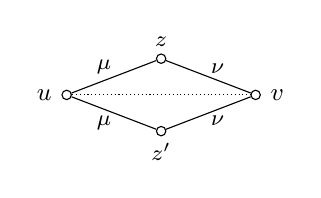
\begin{tikzpicture}[baseline={([yshift=-0.55ex]u.center)},
   every node/.style={font=\footnotesize},vtx/.style={circle,draw,inner sep=1.2pt}]
 \node[vtx,label={[font=\small]left:$u$}] (u) at (0,0) {};
 \node[vtx,label={[font=\small]right:$v$}] (v) at (2.4,0) {};
 \node[vtx,label={[label distance=-1pt]above:$z$}] (z) at (1.2,0.46) {};
 \node[vtx,label={[label distance=-1pt]below:$z'$}] (z2) at (1.2,-0.46) {};
 \draw (u) -- node[above left=-2.5pt] {$\mu$} (z);
 \draw (z) -- node[above right=-2.5pt] {$\nu$} (v);
 \draw (u) -- node[below left=-2.5pt] {$\mu$} (z2);
 \draw (z2) -- node[below right=-2.5pt] {$\nu$} (v);
 \draw[densely dotted] (u) -- (v);
 \end{tikzpicture}
\]
We call such vertices $z$ \defn{witnesses}.
A coloring with this property exists whenever
$|V|\ge n_0(2^k)$, where
$n_0(N)\coloneqq\lceil12N^2\ln(2N)\rceil+3$, since a uniformly random
coloring has it with positive probability
(Lemma~\ref{lem:palette}). These colorings go back to Jipsen, Maddux, and
Tuza~\citep{jipsen-maddux-tuza1995}.

\paragraph{Roadmap.}
In \S\ref{ov:fold}, we construct $2^k$ folds of the reference structure $\mathcal M_0$, each changing the answer of $G_k$ at an unchanged edge.
%
In \S\ref{ov:types}, we show that every circuit gate on $\mathcal M_0$ is constant on each edge-color class and on the diagonal. This allows us to define predictions under each fold.
Boolean operations, including complement, and converse preserve these predictions; only composition can violate them.
%
In \S\ref{ov:twocolors}, we show that, thanks to the two-witness property, each composition can violate the prediction for at most two folds. Since every fold must be detected, any circuit for $G_k$ requires at least $2^{k-1}$ compositions, even with sharing.
\nakamura{violate / detect / notice は重複？（notice は後で定義がある）}

\subsubsection{Folding the reference structure}\label{ov:outline}\label{ov:fold}

We use the reference coloring $\chi$ to define an input structure $\mathcal M_0$ for $G_k$.
On an edge of color $\mu$, we interpret $P_i$ as true exactly when $i\in\mu$, and $Q_i$ exactly when $i\notin\mu$. No input relation holds on loops, which carry the separate label $\id$.
Consequently, a read edge of color $\mu$ accepts exactly witness edges of color $\mu^c$: for distinct $u,v$,
\[
\mathcal M_0 \models G_k(u,v)\iff
\exists z \notin \set{u, v}.\ \chi(u,z)=\chi(u,v)^c.
\]
By the two-witness property, every vertex
has edges of every color, so $G_k$ holds
at every non-loop pair of $\mathcal M_0$.

Fix a vertex $\hub \in V$, the \defn{hub}, and for each color $\mu$ choose $v_\mu$ with $\chi(\hbar,v_\mu)=\mu$.
\nakamura{$\hbar$, $h$, $\hub$ が混在}
%
For each color $\lambda$, let $\chi_\lambda$ be obtained from $\chi$ by recoloring every $\lambda$-colored edge incident to $\hub$ as $\lambda^c$, leaving all other edges unchanged.
Let $\mathcal M_\lambda$ be the input structure induced by $\chi_\lambda$ in the same way as $\mathcal M_0$.
In $\mathcal M_\lambda$, the hub has no edge of color $\lambda$, but the read edge $(\hub,v_{\lambda^c})$ remains unchanged (Figure~\ref{fig:fold}).

\begin{figure}[H]
\begin{minipage}[c]{0.27\linewidth}
\setlength{\abovecaptionskip}{0pt}
\caption[The fold of $\lambda$]{\raggedright The fold of $\lambda$. Only edges at the hub $\hub$ are drawn.}
\label{fig:fold}
\end{minipage}\hfill
\begin{minipage}[c]{0.71\linewidth}
\centering
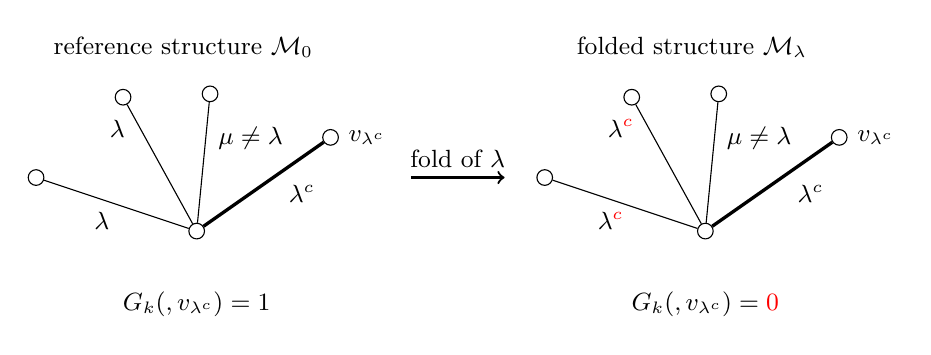
\begin{tikzpicture}[scale=0.85,every node/.style={font=\small},
  vtx/.style={circle,draw,inner sep=2pt}]
\foreach \xs/\col/\val/\name in
  {0/\lambda/1/{reference structure $\mathcal M_0$},
   7.6/\lambda^{\color{red}c}/{\color{red}0}/{folded structure $\mathcal M_\lambda$}}{
\begin{scope}[xshift=\xs cm]
\node at (-0.2,2.75) {\name};
\node[vtx,label={[label distance=2pt]below:$\hub$}] (h) at (0,0) {};
\node[vtx] (a1) at (-2.4,0.8) {};
\node[vtx] (a2) at (-1.1,2.0) {};
\node[vtx] (x) at (0.2,2.05) {};
\node[vtx,label=right:$v_{\lambda^c}$] (v) at (2.0,1.4) {};
\draw (h)--node[below=1pt,pos=0.6] {$\col$} (a1);
\draw (h)--node[left=2pt,pos=0.8] {$\col$} (a2);
\draw (h)--node[right=1pt,pos=0.7] {$\mu\ne\lambda$} (x);
\draw[very thick] (h)--node[below right=0pt,pos=0.62] {$\lambda^c$} (v);
\node at (0,-1.1) {$G_k(\hub,v_{\lambda^c})=\val$};
\end{scope}}
\draw[->,thick] (3.2,0.8)--node[above]{fold of $\lambda$} (4.6,0.8);
\end{tikzpicture}
\end{minipage}
\end{figure}

The read edge $(\hub,v_{\lambda^c})$ requires a $\lambda$-colored edge at $\hub$; the fold removes all such edges. 
\nakamura{辺は削除ではなく、ラベルの反転 (flip)、あるいはラベルの変更か (Fig~\ref{fig:prediction}周辺も同様)}
Hence
\[
\chi_\lambda(\hbar,v_{\lambda^c})
 =\chi(\hbar,v_{\lambda^c})=\lambda^c,\ 
\mathcal M_0\models G_k(\hbar,v_{\lambda^c}),\ 
\mathcal M_\lambda\not\models G_k(\hbar,v_{\lambda^c}).
\]
We call $(\mathcal M_0,\mathcal M_\lambda,(\hub,v_{\lambda^c}))$ the \defn{test} for $\lambda$.
Thus $G_k$ yields $2^k$ tests, one for each color.

\if0
Fix, for each color $\mu$, a vertex $v_\mu$ with $\chi(\hub,v_\mu)=\mu$.
The read edge $(\hub,v_{\lambda^c})$, which the fold of $\lambda$ does not
recolor since $\lambda^c\ne\lambda$, accepts exactly the witness edges of
color $\lambda$. So $G_k(\hub,v_{\lambda^c})$ holds exactly when $\hub$
has an edge of color $\lambda$. Writing $\sem\varphi{\mathcal M}$ also for
the relation that a gate $\varphi$ computes on $\mathcal M$, with value
$\sem\varphi{\mathcal M}(u,v)\in\{0,1\}$ at a pair $(u,v)$, we therefore
get
\[
 \mathcal M_0\xrightarrow{\ \text{fold }\lambda\ }\mathcal M_\lambda
 \quad(\lambda\subseteq[k]),\qquad
 \sem{G_k}{\mathcal M_0}(\hub,v_{\lambda^c})=1\ne0
 =\sem{G_k}{\mathcal M_\lambda}(\hub,v_{\lambda^c}).
\]
We call $\mathcal M_0$, $\mathcal M_\lambda$, and the read edge
$(\hub,v_{\lambda^c})$ the \defn{test} for $\lambda$. So for every color
$\lambda$, every circuit computing $G_k$ has different outputs at the read
edge on $\mathcal M_0$ and on $\mathcal M_\lambda$, although the fold does
not recolor this edge.
\fi


\subsubsection{Circuits see only colors}\label{ov:types}

\paragraph{Color-determined relations.}
A relation $X\subseteq V^2$ is
\defn{color-determined} if
$\chi(u,v)=\chi(u',v') \implies X(u,v)=X(u',v')$ holds.
Here loops carry the separate label $\id$.
Equivalently, $X$ is a union of edge-color
classes, possibly together with the diagonal.
Write $X[\mu]$ for its common value on edges
of color $\mu$, $X[\id]$ for its value on
loops.

Every gate of an arbitrary \CoR\ circuit computes a color-determined relation on $\mathcal M_0$ (Lemma~\ref{lem:tables}).
We can prove this by induction on the
circuit gates. Input relations and constants are
color-determined, while Boolean operations and
converse preserve this property.
The only nontrivial step is composition $X;Y$.

For distinct $u,v$, the two-witness property realizes every pair of colors $\mu,\nu$ along a path $u\xrightarrow{\mu}z\xrightarrow{\nu}v$ with $z\notin\set{u,v}$.
%
The case $z\in\set{u,v}$ depends only on $\chi(u,v)$ and the diagonal values of $X,Y$.
Hence $(X;Y)(u,v)$ depends only on $\chi(u,v)$.
For a loop $(u,u)$, both edges of a path $u-z-u$ have the same color, and every color occurs at every vertex. 
Together with the case $z=u$, this makes $(X;Y)(u,u)$ independent of $u$, completing the induction.


\paragraph{Predicting and noticing a fold.}
A color-determined relation $X$ assigns a value $X[\mu]$ to each color $\mu$.
To predict the effect of a fold, we keep these values fixed and read them at the new edge colors:
\[
\defn{(Prediction)}\quad
X^{(\lambda)}(u,v):=X[\chi_\lambda(u,v)].
\]
Thus a recolored edge reads $X[\lambda^c]$ rather than $X[\lambda]$; all other pairs retain their values.
%
This predicts what a gate would compute if its color-dependent behavior on $\mathcal M_0$ remained unchanged after the fold;
its actual value on $\mathcal M_\lambda$ may differ.

Input relations and constants behave exactly as predicted.
Moreover, Boolean operations and converse commute with prediction
(Proposition~\ref{prop:prediction-commutation}); in particular,
$\overline{X^{(\lambda)}}=(\overline X)^{(\lambda)}$.
Unlike the preservation under embeddings~\eqref{eq:mono} in \S\ref{sec:natural-approaches},
this equality survives unrestricted complement.

Figure~\ref{fig:prediction} compares three operations for any two
distinct colors $\lambda,\mu$: $X$ selects the $\lambda$-colored
edges, and $Y$ the $\mu$-colored edges (both exclude loops).
The thick edge $e=(\hub,v_\mu)$ is unchanged by the fold of
$\lambda$, which removes all $X^{(\lambda)}$-edges at $\hub$.\nakamura{Fig.~\ref{fig:prediction} の表が読めない気がします。列見出しをもう少しちゃんと書くか、caption か本文に説明が欲しいです。
また、Fig.~\ref{fig:prediction} は Fig.~\ref{fig:fold} とほぼ同じにもみえます（あと、塗り替えた辺が Fig.~\ref{fig:prediction} では破線、Fig.~\ref{fig:fold} では実線で、整合性が取れていない）}

\begin{figure}[H]
  \centering
  \begin{minipage}[c]{0.58\linewidth}
    \centering
\begin{tikzpicture}[
      >=Latex,
      vertex/.style={circle,draw,fill=white,inner sep=0pt,minimum size=3.2pt},
      edge/.style={line width=.5pt},
      read/.style={line width=1.05pt},
      folded/.style={draw=red!65!black,densely dashed,line width=.75pt},
      every node/.style={font=\scriptsize},
    ]
      % These four vertices show two of the witnesses; the full arena
      % contains further vertices and satisfies the two-witness property.
      \coordinate (h0) at (0,0);
      \coordinate (v0) at (2.65,0);
      \coordinate (z0) at (1.325,0.98);
      \coordinate (w0) at (1.325,-0.98);
      \draw[read] (h0)--node[below,pos=.54] {$\mu$} (v0);
      \draw[edge] (h0)--node[above left] {$\lambda$} (z0);
      \draw[edge] (h0)--node[below left] {$\lambda$} (w0);
      \draw[edge] (z0)--node[above right] {$\mu$} (v0);
      \draw[edge] (w0)--node[below right] {$\mu$} (v0);
      \node[vertex,label=left:{$\hub$}] at (h0) {};
      \node[vertex,label=right:{$v_\mu$}] at (v0) {};
      \node[vertex,label=above:{$z$}] at (z0) {};
      \node[vertex,label=below:{$z'$}] at (w0) {};
      \node[font=\small] at (.1, 1.2) {$\mathcal M_0$};
      \draw[-{Latex[length=2mm]},line width=.7pt]
        (3.4,0)--node[above] {fold $\lambda$} (4.85,0);
      \begin{scope}[xshift=5.30cm]
        \coordinate (h1) at (0,0);
        \coordinate (v1) at (2.65,0);
        \coordinate (z1) at (1.325,0.98);
        \coordinate (w1) at (1.325,-0.98);
        \draw[read] (h1)--node[below,pos=.54] {$\mu$} (v1);
        \draw[folded] (h1)--node[above left,black] {$\lambda^c$} (z1);
        \draw[folded] (h1)--node[below left,black] {$\lambda^c$} (w1);
        \draw[edge] (z1)--node[above right] {$\mu$} (v1);
        \draw[edge] (w1)--node[below right] {$\mu$} (v1);
        \node[vertex,label=left:{$\hub$}] at (h1) {};
        \node[vertex,label=right:{$v_\mu$}] at (v1) {};
        \node[vertex,label=above:{$z$}] at (z1) {};
        \node[vertex,label=below:{$z'$}] at (w1) {};
        \node[font=\small] at (.1, 1.2) {$\mathcal M_\lambda$};
      \end{scope}
    \end{tikzpicture}
  \end{minipage}\hfill%
  \begin{minipage}[c]{0.40\linewidth}
    \centering
    {\footnotesize
    \renewcommand{\arraystretch}{1.16}%
    \begin{tabular}{@{}lccc@{}}
      \toprule
      Operation & Predicted & Actual & Notice? \\
      \midrule
      $X;Y$         & $1$ & $0$ & Yes \\
      $X\cup Y$     & $1$ & $1$ & No \\
      $\overline X$ & $1$ & $1$ & No \\
      \bottomrule
    \end{tabular}}
  \end{minipage}
  \caption{At $e=(\hub,v_\mu)$, only composition notices the fold of $\lambda$.
    Only two witness paths are shown; all $\lambda$-edges at $\hub$ are recolored to $\lambda^c$.}
  \label{fig:prediction}
\end{figure}

\if0
An operation \defn{notices} a fold at given color-determined
operands if applying it after prediction differs from predicting its
result. In Figure~\ref{fig:prediction}, composition notices the fold:
$X^{(\lambda)};Y^{(\lambda)}\ne(X;Y)^{(\lambda)}$.
Union and complement do not notice it; indeed, Proposition~\ref{prop:prediction-commutation}
shows that no Boolean operation or converse can ever notice a fold.
\fi

An operation \defn{notices} a fold at given
color-determined operands if applying it to
their predictions differs from predicting
its result. In Figure~\ref{fig:prediction}, composition notices
the fold at $e$, since
\[
  e\notin\bigl(X^{(\lambda)};Y^{(\lambda)}\bigr)
  \quad \text{and} \quad
  e\in(X;Y)^{(\lambda)}.
\]
By contrast, union and complement do not
notice the fold. More generally, no Boolean
operation or converse can notice any fold
(Proposition~\ref{prop:prediction-commutation}).

Every fold must be noticed by some composition gate.
Let $C$ be a \CoR\ circuit such that $C\equiv G_k$.
If no composition gate notices the fold of $\lambda$,
then, since $(\hub,v_{\lambda^c})$ is unchanged,
Lemma~\ref{lem:unnoticed} gives
\[
  \mathcal M_0\models C(\hub,v_{\lambda^c})
  \quad\Longleftrightarrow\quad
  \mathcal M_\lambda\models C(\hub,v_{\lambda^c}).
\]
This contradicts $C\equiv G_k$, since
$\mathcal M_0\models G_k(\hub,v_{\lambda^c})$
but $\mathcal M_\lambda\not\models G_k(\hub,v_{\lambda^c})$.

\if0
Every fold must be noticed by some composition gate.
Now let $C$ be any circuit computing $G_k$.
If no composition gate notices the fold of
$\lambda$, Lemma~\ref{lem:unnoticed} implies that the output
on $\mathcal M_\lambda$ is the prediction
of the output on $\mathcal M_0$.
Since the test edge $e_\lambda=(\hub,v_{\lambda^c})$ is unchanged,
\[
\sem{C}{\mathcal M_\lambda}(e_\lambda)
=
\bigl(\sem{C}{\mathcal M_0}
\bigr)^{(\lambda)}(e_\lambda)
=
\sem{C}{\mathcal M_0}(e_\lambda),
\]
contradicting the test for $\lambda$, whose outputs are $0$ on $\mathcal M_{\lambda}$ and $1$ on $\mathcal M_0$.
\fi


\subsubsection{Each composition notices at most two folds}\label{ov:twocolors}

We now show that any composition $X;Y$ of color-determined relations
notices at most two folds (Lemma~\ref{lem:local}). The two-witness
property first rules out noticing at pairs away from the hub.

\paragraph{Away from the hub (Figure~\ref{fig:notice}).}
At pairs $(u,v)$ with $u,v\ne\hub$, composition agrees with
prediction.
Figure~\ref{fig:notice} uses the same coloring, operands $X,Y$, and fold
as Figure~\ref{fig:prediction}, but observes $e'=(u,v_\mu)$.

\begin{figure}[H]
  \centering
  \begin{tikzpicture}[
    >=Latex,
    every node/.style={font=\scriptsize},
    vtx/.style={circle,draw,fill=white,inner sep=1.5pt},
    edge/.style={line width=.55pt},
    recolored/.style={red!75!black,densely dashed,line width=.85pt},
    surviving/.style={line width=1.15pt},
    read/.style={densely dotted,line width=.55pt},
  ]
    % Same four vertices and positions before and after folding.
    % u is the vertex z of Figure 2, and w is its alternative witness.
    \begin{scope}
      \coordinate (u0) at (0,0);
      \coordinate (v0) at (2.65,0);
      \coordinate (h0) at (1.325,.98);
      \coordinate (w0) at (1.325,-.98);
      \draw[read] (u0)--node[below,pos=.57] {$\mu$} (v0);
      \draw[edge] (u0)--node[above left] {$\lambda$} (h0);
      \draw[edge] (h0)--node[above right] {$\mu$} (v0);
      \draw[surviving] (u0)--node[below left] {$\lambda$} (w0);
      \draw[surviving] (w0)--node[below right] {$\mu$} (v0);
      \node[vtx,label=left:{$u$}] at (u0) {};
      \node[vtx,label=right:{$v_\mu$}] at (v0) {};
      \node[vtx,label=above:{$\hub$}] at (h0) {};
      \node[vtx,label=below:{$w$}] at (w0) {};
      \node[font=\small] at (.1, 1.2) {$\mathcal M_0$};
    \end{scope}
    \draw[-{Latex[length=2mm]},line width=.7pt]
      (3.30,0)--node[above] {fold $\lambda$} (4.65,0);
    \begin{scope}[xshift=5.25cm]
      \coordinate (u1) at (0,0);
      \coordinate (v1) at (2.65,0);
      \coordinate (h1) at (1.325,.98);
      \coordinate (w1) at (1.325,-.98);
      \draw[read] (u1)--node[below,pos=.57] {$\mu$} (v1);
      \draw[recolored] (u1)--node[above left,black] {$\lambda^c$} (h1);
      \draw[edge] (h1)--node[above right] {$\mu$} (v1);
      \draw[surviving] (u1)--node[below left] {$\lambda$} (w1);
      \draw[surviving] (w1)--node[below right] {$\mu$} (v1);
      \node[vtx,label=left:{$u$}] at (u1) {};
      \node[vtx,label=right:{$v_\mu$}] at (v1) {};
      \node[vtx,label=above:{$\hub$}] at (h1) {};
      \node[vtx,label=below:{$w$}] at (w1) {};
      \node[font=\small] at (.1, 1.2) {$\mathcal M_\lambda$};
    \end{scope}
  \end{tikzpicture}
  \caption{Away from the hub, the fold invalidates the path through $\hub$
    but leaves the second witness path through $w$ unchanged.
    Only these two witness paths are shown.}
  \label{fig:notice}
\end{figure}

In $\mathcal M_0$, both paths have colors $(\lambda,\mu)$.
After the fold, the path through $\hub$ is invalidated but the path through $w$ survives.
Hence:
$(X^{(\lambda)};Y^{(\lambda)})(e')
=1
=(X;Y)^{(\lambda)}(e')$.

More generally, between any distinct $u,v\ne\hub$, the two-witness
property preserves every two-color path pattern via a witness other
than $\hub$. Loops away from $\hub$ retain edges of every color, and
endpoint witnesses are unchanged. Thus composition cannot violate
prediction away from the hub.

\paragraph{At the hub (Figure~\ref{fig:prediction} revisited).}

Only pairs involving $\hub$ remain.
In Figure~\ref{fig:prediction}, $X$ holds only on $\lambda$ and
$Y$ only on $\mu$, where $\lambda\ne\mu$.
Their composition notices the folds of
$\lambda$ and $\mu$ at $(\hub,v_\mu)$ and
$(v_\lambda,\hub)$, respectively.

Why can it not notice a third fold?
To notice $\lambda$ at $(\hub,v)$, $X$ must
hold on $\lambda$ and no other off-diagonal
color. Indeed, if $X[\nu]=1$ for some
$\nu\ne\lambda$ and $Y[\tau]=1$ for some
color $\tau$, the two-witness property
supplies a path
$\hub\xrightarrow{\nu}z\xrightarrow{\tau}v$
that survives the fold of $\lambda$.
Thus $z$ remains a witness for
$(X^{(\lambda)};Y^{(\lambda)})(\hub,v)$.
%
Likewise, noticing a distinct fold $\mu$
at $(u,\hub)$ requires $Y$ to hold only
on $\mu$. Hence noticing two distinct
folds forces $X$ and $Y$ to be supported
on $\{\lambda\}$ and $\{\mu\}$, respectively.
No third color occurs in either support,
and their supports are disjoint, ruling out
an additional fold noticed at $(\hub,\hub)$.
If $X$ and $Y$ share a color instead,
all possible noticed folds must coincide.
Thus $X;Y$ notices at most two folds.

\paragraph{Summary.}
Every one of the $2^k$ folds requires a noticing composition gate
(\S\ref{ov:types}), whereas each distinct composition gate notices at
most two (Lemma~\ref{lem:local}). Hence $2^k\le 2\gcost C$,
proving the lower bound of Theorem~\ref{thm:main} even with sharing.
% For these tests, the factor two is tight (Proposition~\ref{prop:promise}).



% Requires mathrsfs for \mathscr{P} and TikZ (arrows.meta) for Figure~\ref{fig:reverse-fold}.
\subsection{Further results}\label{sec:additional-results}
In \S\ref{sec:overview}, we explained how folds of a reference structure
prove our main theorem. We now use this approach to establish further
exponential succinctness gaps: from $\FOthree$ to $\FOtwo$, from
$\CoR$ to $\FOtwo$, and from three-attribute relational algebra to
matrix query languages. To explain these extensions, we first summarize
the counting argument of \S\ref{sec:overview}.

Recall that the folds in \S\ref{sec:overview} are indexed by colors $\lambda\in\Lambda=2^{[k]}$.
For a circuit $C \equiv G_k$,
let $D_g\subseteq\Lambda$ be the set of colors whose folds are noticed by gate $g$.
Every color belongs to some $D_g$: otherwise, the circuit
could not detect the change at the read edge left unchanged by that
fold (\S\ref{ov:types}). Thus $\bigcup_{g\in C}D_g=\Lambda$, and
counting gives
\begin{equation}\tag{$\dagger$}\label{eq:fold-counting}
  2^k\le \sum_{g\in C}|D_g|.
\end{equation}
For \CoR, Boolean operations and converse notice no folds, while each
composition notices at most two (\S\ref{ov:twocolors}). Hence
$\sum_{g\in C}|D_g|\le 2\gcost C$, recovering Theorem~\ref{thm:main}.
The applications below use the same counting argument, with different
bounds on the folds noticed by the target operations and, when needed,
a different reference structure.

\paragraph{\texorpdfstring{{\boldmath\FOthree\ to \FOtwo}}{FO3 to FO2}.}
The same query $G_k$ is also \FOtwo-definable: the DNF expansion in
\S\ref{sec:main-results} gives
\[
 G_k(x,y)\equiv\bigvee_{A\subseteq[k]}
 \bigl[H_A(x,y)\land\exists y\,H_{A^c}(x,y)\bigr]
\]
where $H_A$ is \FOtwo-definable.
Here the quantifier binds $y$ only in the second conjunct.
\begin{restatable}[Exponential lower bound from \FOthree\ to \FOtwo\proofref{sec:FOtwo}]{theorem}{sentencebounds}\label{cor:sentences}
For every $k\ge1$,
every \FOtwo\ formula $\varphi$ such that $\varphi\equiv G_k$ has at least $2^k$ quantifiers.

%The bound holds even if $\varphi$ and $G_k$ agree only on finite structures.
\end{restatable}
The displayed expansion uses exactly $2^k$ quantifiers, so the bound
is tight. To our knowledge, this is the first exponential succinctness
gap from \FOthree\ to \FOtwo\ over general finite structures. The gap
also holds for sentences. On pure finite linear orders, by contrast,
\FOthree\ sentences admit polynomial-size \FOtwo\ translations
\citep{grohe-schweikardt2005}, while Vinall-Smeeth's exponential
separations over general structures start at three target variables
\citep{vinall-smeeth2024} (see \S\ref{sec:relwork}).

The same reference structure $\mathcal M_0$ and folds from \S\ref{sec:overview} suffice.
Indeed, regard each \FOtwo\ subformula $\psi$ as a binary relation
$X_\psi$ of assignments to $(x,y)$, with any unused coordinate treated
as a dummy. Quantifying a variable is then a special case of relational
composition:
\[
  X_{\exists y\,\psi}=X_\psi;\one,
  \qquad
  X_{\exists x\,\psi}=\one;X_\psi.
\]
Thus their assignment relations remain color-determined on $\mathcal M_0$,
just like the CoR gate values in \S\ref{sec:overview}.
Since one operand of each composition is $\one$, each quantifier can
notice at most one fold (\S\ref{ov:twocolors}), rather than the two
possible for general composition. Atomic formulas and Boolean
connectives notice none; universal quantifiers are handled by
complement. The counting inequality~\eqref{eq:fold-counting} therefore
requires at least $2^k$ quantifiers. We also obtain a lower bound of $k2^k$ relation-atom occurrences and
optimal tree size $\Theta(k2^k)$, for both queries and sentences
(\S\ref{sec:sentences}).

For \CoR\ itself, we also determine the optimal tree size of $G_k$
as $(2+o(1))k2^k$, whereas its optimal circuit size is $\Theta(2^k)$
(Theorem~\ref{thm:tree}).

\paragraph{\texorpdfstring{{\boldmath\CoR\ to \FOtwo}}{CoR to FO2}.}
An exponential succinctness gap also occurs from \CoR\ to \FOtwo.
We need a different query, since $G_k$ already requires exponentially
many \CoR\ compositions. Put $\mathscr P_i^1\coloneqq\id\cap P_i$
and $\mathscr P_i^0\coloneqq\id\cap\overline{P_i}$, and let
$\vartheta_A(u)\coloneqq\bigwedge_{i\in A}P_i(u,u)\land
\bigwedge_{i\notin A}\neg P_i(u,u)$ for $A\subseteq[k]$.
Consider the following linear-size \CoR\ term and its \FOtwo\ expansion:
\[
\defn{\CoR}:
 U_k \coloneqq R;\bigcap_{i=1}^k
 \left[(\mathscr P_i^0;\one;\mathscr P_i^0)
 \cup(\mathscr P_i^1;\one;\mathscr P_i^1)\right]
 \longrightarrow
\defn{\FOtwo}:
 \bigvee_{A\subseteq[k]}
 \left[\vartheta_A(y)\land\exists y\,
    (R(x,y)\land\vartheta_A(y))\right]
\]
Thus $U_k$ asks whether $x$ has an $R$-successor with the same
$k$-bit loop pattern as $y$.
\begin{restatable}[Exponential lower bound from \CoR\ to \FOtwo\proofref{sec:reverse}]{proposition}{reverse}\label{prop:reverse}
For every $k\ge1$, every \FOtwo\ formula
$\varphi$ such that $\varphi\equiv U_k$ has at least
$2^k$ quantifiers.
% The bound holds even if $\varphi$ and $U_k$ agree only on finite structures.
\end{restatable}

The displayed expansion uses exactly $2^k$ quantifiers, so the bound
is tight.
%
For the lower bound, take a new reference structure $\mathcal W_0$
with several vertices of each loop pattern and a hub $h$ having
$R$-successors of every pattern (Figure~\ref{fig:reverse-fold}).
The fold of $A\subseteq[k]$ deletes all $R$-edges from $h$ to
vertices of pattern $A$.
Thus $U_k(h,y_A)$ changes from true to false
for a vertex $y_A$ of pattern $A$, even when $(h,y_A)$ is unchanged.

\begin{figure}[!htbp]
\centering
\begin{tikzpicture}[
  >=Stealth,
  every node/.style={font=\small},
  patternclass/.style={draw=black!55, fill=black!3,
      rounded corners=2pt, minimum width=2.9cm, minimum height=.78cm},
  member/.style={circle, fill=black, inner sep=1.55pt},
  testmember/.style={circle, fill=black!50, inner sep=1.55pt},
  redge/.style={->, semithick, shorten >=2pt},
]
\begin{scope}
  \node[font=\bfseries\small] at (0.5, 1.0) {Reference $\mathcal W_0$};
  \node[draw,circle,inner sep=2pt] (h0) at (.20,0) {$h$};
  \node[patternclass] at (4.10,.69) {};
  \node[font=\scriptsize,anchor=south] at (4.10,1.10) {pattern $A$};
  \node[member,label={[font=\scriptsize]right:$z_A$}] (za0) at (3.54,.64) {};
  \node[testmember,label={[font=\scriptsize]right:$y_A$}] at (4.66,.64) {};
  \node[patternclass] at (4.10,-.78) {};
  \node[font=\scriptsize,anchor=south] at (4.10,-.37) {pattern $B\ne A$};
  \node[member,label={[font=\scriptsize]right:$z_B$}] (zb0) at (3.60,-.84) {};
  \draw[redge] (h0) -- (za0);
  \draw[redge] (h0) -- (zb0);
  \node[font=\scriptsize] at (2.78,-1.62) {$U_k(h,y_A)=1$};
\end{scope}
\begin{scope}[xshift=7.1cm]
  \node[font=\bfseries\small] at  (0.5, 1.0) 
  {Folded $A$: $\mathcal W_A$};
  \node[draw,circle,inner sep=2pt] (h1) at (.20,0) {$h$};
  \node[patternclass] at (4.10,.69) {};
  \node[font=\scriptsize,anchor=south] at (4.10,1.10) {pattern $A$};
  \node[member,label={[font=\scriptsize]right:$z_A$}] (za1) at (3.54,.64) {};
  \node[testmember,label={[font=\scriptsize]right:$y_A$}] at (4.66,.64) {};
  \node[patternclass] at (4.10,-.78) {};
  \node[font=\scriptsize,anchor=south] at (4.10,-.37) {pattern $B\ne A$};
  \node[member,label={[font=\scriptsize]right:$z_B$}] (zb1) at (3.60,-.84) {};
  \draw[redge,dashed,black!35] (h1) -- (za1);
  \node[font=\large, text=black!70] at (2.25,.39) {$\times$};
  \draw[redge] (h1) -- (zb1);
  \node[font=\scriptsize] at (2.78,-1.62) {$U_k(h,y_A)=0$};
\end{scope}
\end{tikzpicture}
\caption{The fold of $A$ removes all $R$-edges from $h$ to vertices of loop pattern $A$ (schematic).}
\label{fig:reverse-fold}
\end{figure}

The original folds cannot give this separation: on their reference
structure, every composition notices at most two folds, ruling out a
short \CoR\ term that distinguishes all those tests. In the new
structure, the outer composition of $U_k$ can notice all $2^k$ folds,
whereas each \FOtwo\ quantifier, viewed as a projection, still notices
at most one. The latter bound uses redundant representatives of each
atomic pair type. Applying the same counting argument~\eqref{eq:fold-counting}
to the new tests proves the lower bound (\S\ref{sec:reverse}).

\paragraph{Arity elimination in matrix query languages.}
Brijder~et~al.\ compared two formalisms for semiring-valued queries:
ARA$(3)$, which allows intermediate tables with up to three columns,
and MATLANG, which computes with matrices, vectors, and scalars.
They showed that the two have the same expressive power when inputs
and outputs have at most two columns~\cite{brijder2022}.
Their translation from ARA$(3)$ to MATLANG can grow exponentially,
but whether this blowup is unavoidable was left open~\citep[p.~9]{brijder2019}.
We establish an exponential lower bound using a semiring-valued
analogue of our hard query $G_k$.

Let $\mathfrak S=(S,\oplus,\otimes,0_S,1_S)$ be a commutative semiring,
with input relations $P_i,Q_i:V^2\to S$. Define
\[
  \mathcal G_k(x,y)\coloneqq
  \bigoplus_{z\in V}\ \bigotimes_{i=1}^k
  \Bigl[(P_i(x,y)\otimes Q_i(x,z))
  \oplus(Q_i(x,y)\otimes P_i(x,z))\Bigr].
\]
This query has an ARA$(3)$ expression of size $O(k)$: all $k$
conditions are combined over $(x,y,z)$ before $z$ is aggregated away.
Over Boolean annotations ($S=\mathbb B$, with $\oplus=\lor$ and
$\otimes=\land$), $\mathcal G_k$ specializes to $G_k$.

In MATLANG, the usual semiring matrix--vector (mv) and matrix--matrix
(mm) products take the form
\[
  (A \cdot v)(x) \coloneqq \smash{\bigoplus_{z\in V}} A(x,z)\otimes v(z)
  \quad\text{(mv)},\qquad
  (A \cdot B)(x,y) \coloneqq \smash{\bigoplus_{z\in V}} A(x,z)\otimes B(z,y)
  \quad\text{(mm)}.
\]

Both eliminate their aggregated index immediately.
The DNF of \S\ref{sec:main-results} also gives an explicit MATLANG
representation of $\mathcal G_k$. Here $H_A$ is obtained from the expression in \S\ref{sec:main-results}
by replacing intersections with pointwise $\otimes$, and
$\mathbf 1_S$ is the all-$1_S$ column vector. Then
\[
  \mathcal G_k(x,y)=\smash{\bigoplus_{A\subseteq[k]}}
       H_A(x,y)\otimes (H_{A^c}\mathbf \cdot \mathbf{1}_S)(x).
\]

This uses $2^k$ mv products, together with row broadcasting and
entrywise operations; more general computations may also use mm
products and shared intermediate results.
For a circuit $C$, let $\mvcount C$ count matrix--vector and
vector--matrix aggregations, and $\mmcount C$ count matrix--matrix
aggregations, with shared gates counted once. All other permitted
operations are free.

For a concrete non-Boolean case, consider the natural and integer
min--plus semirings
$\mathsf{Trop}_D \coloneqq (D\cup\{+\infty\},\min,+,+\infty,0)$,
where $D\in\{\mathbb N,\mathbb Z\}$.

\begin{restatable}[Tropical arity-elimination overhead\proofref{sec:matrix}]{theorem}{tropicalmatrixbounds}\label{thm:tropical-matrix}
For every $k\ge1$ and $\mathfrak S\in\{\mathsf{Trop}_{\mathbb N},\mathsf{Trop}_{\mathbb Z}\}$,
the query $\mathcal G_k$ has an ARA$(3)$ expression of size $O(k)$,
but every typed matrix circuit $C$ over $\mathfrak S$ computing it
on all finite inputs satisfies $\mvcount C+3\mmcount C\ge2^k$.
\end{restatable}
The lower bound holds even with arbitrary uniform entrywise functions
and aggregation kernels. Its proof uses the fold-counting principle
\eqref{eq:fold-counting} (\S\ref{sec:matrix}).

The argument extends uniformly beyond tropical matrices.
Examples include the Boolean semiring $(\{0,1\},\lor,\land)$
and the max--min semiring $([0,1],\max,\min)$.
It also covers integer max--plus
$(\mathbb Z\cup\{-\infty\},\max,+)$ and, for each fixed $b\ge1$,
finite-set annotations $(2^{[b]},\cup,\cap)$ and $b$-dimensional
min--plus $\mathsf{Trop}_{\mathbb Z}^{b}$.
One property covers all these examples: \emph{finite join breadth},
meaning that every finite join is determined by a bounded number
of its summands. It bounds how many folds an aggregation can notice,
giving exponential lower bounds for every fixed nontrivial
commutative idempotent semiring of finite join breadth
(Theorem~\ref{cor:matrix}). Over Boolean matrices, we also obtain
the sharper bound $\mvcount C+2\mmcount C\ge2^k$.
Positive computations over nonidempotent semirings such as
$(\mathbb N,+,\times)$ are handled separately by Booleanization
(\S\ref{sec:positive}).

\paragraph{Robustness: closure and randomization.}

The lower bound persists even when \CoR\ is extended with reflexive–transitive closure 
$X^* \coloneqq \bigcup_{m\ge 0}X^m$,
which can be evaluated in $O(n^\omega)$ time~\citep{fischer-meyer1971,munro1971,furman1970}.
Each closure gate notices at most one fold.


\begin{restatable}[Closure does not help\proofref{sec:closure}]{proposition}{closure}\label{prop:star}
Let $C$ be a \CoR\ circuit with closure gates $(-)^*$
and let $g_*(C)$ count its distinct closure gates.
For every $k \ge 1$,
if $C\equiv G_k$, then $2\gcost C+g_*(C)\ge2^k$.
\end{restatable}

The lower bound also extends to bounded-error randomized circuits, even when circuits are specialized to each sufficiently large domain size.

\begin{restatable}[Fixed sizes and bounded error\proofref{sec:query-bounds}]{corollary}{randomizedbounds}\label{cor:randomized}

For some constant $c>0$, for every $k\ge 1$, $n\ge ck4^k$, and $0\le\varepsilon<1/2$, every input-independent distribution of size-specific \CoR\ circuits whose output at each pair $(u,v)$ is correct with probability at least $1-\varepsilon$ on every $n$-element input satisfies
\[
\mathbb E[g_{;}(C)]\ge(1-2\varepsilon)2^{k-1}.
\]
\end{restatable}

\subsection{Related work}\label{sec:relwork}

\paragraph{History of \CoR.}
\CoR\ predates first-order logic as a formal
system. De Morgan introduced relational composition and converse in his
work on the syllogism in the 1850s and 1860s
\citep{demorgan1856,demorgan1864}; Peirce developed the logic of
relatives~\citep{peirce1870,peirce1880}, and Schr\"oder devoted a volume
to it in 1895~\citep{schroeder1895}. This was before first-order logic
was isolated in Hilbert's lectures and Hilbert and Ackermann's
textbook~\citep{hilbert-lectures,hilbert-ackermann1928,moore1988}.
The central expressiveness problem was whether every quantified statement
about relations could be \emph{condensed} into this variable-free calculus.
Schr\"oder claimed that it could~\citep[p.~551]{schroeder1895}, but
Korselt found a counterexample, published by L\"owenheim in
1915~\citep{loewenheim1915,loewenheim1967}. In modern terms, the \FOfour\ sentence
$
\forall a_1\,a_2\,a_3\,a_4.\bigvee_{i,j; i\neq j} a_i = a_j
$
states that the domain has at most three elements, but is expressible
neither in \FOthree\ nor by a \CoR\ equation.

Tarski raised the expressiveness question in 1941~\citep{tarski1941}
and, according to Tarski and Givant, soon obtained the three-variable
characterization: \CoR\ defines exactly the \FOthree-definable binary
queries. A full proof appeared only in their 1987
monograph~\citep{tarski-givant1987}; see
also~\citep{maddux2006}. For historical accounts, see
\citep{pratt1992,maddux1991,burris-legris,brady2000}.
Their original recursive translation~\citep[\S3.9]{tarski-givant1987}
did not analyze its size. A straightforward bottom-up translation using
DNF conversion~\citep{hilbert-ackermann1928,kleene1952,schoening1989}
and quantifier elimination by relational composition gives a
single-exponential upper bound (Appendix~\ref{app:classical-translation});
the reverse \CoR-to-\FOthree\ translation is linear.

\paragraph{Relational computation and quantifier elimination.}
The operations underlying \CoR\ have long served as computational
primitives, often in calculi distinct from full \CoR.
Copilowish gave a matrix-based treatment of the calculus over finite
domains~\citep{copilowish1948}, while Levien and Maron applied relational
operations to retrieval and inference
\citep{levien-maron1965,levien-maron1967,levien1969}.
Codd's relational algebra laid the foundations of database querying
\citep{Codd1970,Codd1972}, followed by work on relational-expression
equivalence, optimization, and efficient join evaluation
\citep{aho-sagiv-ullman1979equiv,aho-sagiv-ullman1979opt,
SelingerEtAl1979,yannakakis1981}.
Binary relational-expression evaluation became an algorithmic subject
\citep{hunt-szymanski-ullman1974,hunt-szymanski-ullman1977,
szymanski-ullman1975,szymanski-ullman1977}, with applications to parsing
and recursive database queries
\citep{sippu-soisalon-soininen1985,grahne-sippu-soisalon-soininen1987,
grahne-sippu-soisalon-soininen1991}.
Related algebras also appear in relational programming, temporal
reasoning, database execution, and graph querying
\citep{maclennan1981,montanari1974,allen1983,boncz-kersten1999,
cruz-mendelzon-wood1987,FletcherEtAl2015,HellingsEtAl2021,
HellingsEtAl2022}.

A second line of work exploits relational composition as existential
quantifier elimination, using matrix multiplication for fast evaluation.
Early examples include transitive closure
\citep{furman1970,fischer-meyer1971,munro1971,oneil-oneil1973,
galil-margalit1993} and algorithms for triangles, cliques, cycles,
and small subgraphs
\citep{itai-rodeh1978,nesetril-poljak1985,alon-yuster-zwick1997,
kloks-kratsch-mueller2000,eisenbrand-grandoni2004,yuster-zwick2004}.
Already in 1977, Chandra and Merlin studied generalized join--project
operations and their evaluation by rectangular Boolean matrix
multiplication~\citep{ChandraMerlin1977}.
Williams's algorithm for prenex first-order graph properties
\citep{Williams2014} can be viewed in the same algebraic framework:
DNF-based quantifier elimination yields ordinary \CoR\ composition
for three quantifiers and typed composition over tuples for larger
prenex formulas, evaluated using rectangular matrix multiplication
(as in \citep{ChandraMerlin1977}).
Gao and Impagliazzo\ \citep{GaoImpagliazzo2019} also treated general
\FOthree\ formulas, beyond prenex normal form, using matrix-based
evaluation.
Related techniques appear in first-order graph algorithms
\citep{BringmannFischerKunnemann2019} and database join--project
and join--aggregate evaluation
\citep{DeepHuKoutris2020,hu-yi2020,Hu2024,AboKhamisHuSuciu2025}.
Most directly, our earlier work used the \FOthree-to-\CoR\ translation
for truly subcubic \FOthree\ model checking
\citep{nakamura-uezato2027}.

\paragraph{Succinctness results.}
Nakamura proved exponential lower bounds for positive \CoR\ and
$\Sigma_1\CoR$, even for circuits, and a superpolynomial separation over
one binary relation~\citep[\S6]{nakamura2022}. The case of full \CoR\
remained open (see \S\ref{sec:natural-approaches}). In our earlier
work~\citep[Corollary~40]{nakamura-uezato2027}, we ruled out
polynomial-time \FOthree-to-\CoR\ translations under the 3-OV
hypothesis, but not the existence of small equivalent representations.
Theorem~\ref{thm:main} gives an unconditional exponential lower bound
even for \CoR\ circuits, while Theorem~\ref{thm:fixed-vocabulary}
gives tight subexponential circuit bounds over one binary relation.

On finite linear orders with no additional relations, Grohe and Schweikardt proved a polynomial-size translation from \FOthree\ to \FOtwo\ sentences~\citep[Theorem~4.3]{grohe-schweikardt2005}. Since \FOtwo\ translates linearly into \CoR, this also yields polynomial-size \CoR\ equations. By contrast, our exponential succinctness gaps from \FOthree\ to both \FOtwo\ and \CoR\ hold even for sentences over general finite structures.
%
They also showed that full first-order logic is exponentially more
succinct than \FOthree\ on the same orders, already witnessed by
\FOfour~\citep[Theorem~5.3]{grohe-schweikardt2005}. The short \FOfour\
formulas combine divide-and-conquer for distances~\citep{savitch1970}
with the classical quantifier-based abbreviation trick, which avoids
duplicating recursive subformulas
\citep{fischer-rabin1974,stockmeyer1974,ferrante-rackoff1979,compton-henson1990,vorobyov1996,stockmeyer-meyer2002}.
The \FOthree\ lower bound draws on Adler--Immerman formula-size
games~\citep{adler-immerman2003}. However, the resulting distance
predicates admit linear-size \CoR\ circuits by repeated squaring,
$S_{i+1}=S_i;S_i$; our lower bound holds even with such sharing.

Vinall-Smeeth established exponential succinctness gaps from
$\mathrm{FO}^{\ell+1}$ to $\mathrm{FO}^{\ell}$ for every $\ell\ge 3$,
using higher-arity (non-binary) relations~\citep[Theorem~2]{vinall-smeeth2024}.
Our result establishes the \FOthree-to-\FOtwo\ case over binary
signatures, with an exponential lower bound on the number of
quantifiers. The linear \FOtwo-to-\CoR\ translation was already
known~\citep{nakamura2022}, while Proposition~\ref{prop:reverse}
gives an exponential gap in the reverse direction.

\paragraph{Lower-bound methods.}
As explained in \S\ref{sec:natural-approaches}, the witness-crossing
argument underlying Nakamura's formula-size-game proof for $\Sigma_1\CoR$
\citep{adler-immerman2003,nakamura2022} relies on embeddings, which fail
under unrestricted complement. We also considered other standard
lower-bound techniques, but their usual resource measures do not directly
fit our setting. Formula-size games
\citep{grohe-schweikardt2005,french2013,hella-vilander2019},
Ehrenfeucht--Fra\"{\i}ss\'e and pebble games
\citep{fraisse1954classif,ehrenfeucht1961,immerman1982,libkin2004},
and multi-structural games
\citep{immerman1981,fagin2021,carmosino2024} address formula size,
quantifier depth, variable count, or quantifier number, rather than the
number of distinct composition gates in circuits with sharing. Indeed,
$G_k$ has only one quantifier and admits a \CoR\ expression of
composition depth one; the issue is the \emph{number} of compositions.
Monotone-circuit lower bounds~\citep{razborov1985,alon-boppana1987}
are natural candidates for our positive query, but equivalent full-\CoR\
circuits may use unrestricted complement. Switching-lemma and
random-restriction methods~\citep{hastad1986} typically exploit
shallow Boolean-circuit structure, whereas we impose no restrictions on
Boolean nesting and charge only compositions.

Communication complexity suggests further approaches. Rank,
discrepancy, and Karchmer--Wigderson techniques
\citep{mehlhorn-schmidt1982,kushilevitz-nisan1997,karchmer-wigderson1990,jukna2012}
do not directly bound compositions when Boolean operations are free.
For example, set disjointness has rank $2^k$, yet its $1$-entries form
the complement of a union of only $k$ rectangles. Alternating existential
and universal witness tests also resemble the nondeterministic and
co-nondeterministic levels of the communication polynomial hierarchy
\citep{babai-frankl-simon1986,goos-pitassi-watson2018}, but we know of
no direct transfer of lower bounds to our circuit model. These approaches did not yield the required composition-count bound.

Our proof instead draws on the affine-plane and random colorings of
Jipsen, Maddux, and Tuza~\citep{jipsen-maddux-tuza1995}, which, as
explained in the technical overview, already yield the two-witness
property needed here. The new ingredient is our fold-based argument:
it bounds how many local folds each distinct operation can notice,
even with unrestricted complement and circuit sharing.

\subsection{Organization}
Section~\ref{sec:aggregation} fixes semantics and resource measures.
Section~\ref{sec:preservation} builds the reference structure, proves
that unnoticed folds leave a circuit's values as predicted and that each
composition notices at most two folds, and states the test--cost
theorem. Section~\ref{sec:logical} supplies the tests for $G_k$ and
proves Theorem~\ref{thm:main} together with the other bounds for
relational circuits: equations, fixed sizes and bounded error, circuits
without converse, domain size, random inputs, and closure.
Section~\ref{sec:fixed-vocabulary} proves the tight fixed-vocabulary
circuit bounds and derives the model-checking application.
Section~\ref{sec:FOtwo} transfers the bound to quantifiers, determines
the minimum term size, and proves Theorem~\ref{cor:sentences} and
Proposition~\ref{prop:reverse}. Section~\ref{sec:matrix} gives a concrete ARA$(3)$ query,
formalizes typed matrix circuits, and extends the fold analysis to
semiring-valued aggregation.
The appendices
give explicit two-witness colorings, the term-size charging argument and
the sharpness of the fold tests, the directed construction for circuits
without converse, and the classical single-exponential translation.

